The software architecture may be of interest to developers of tree editors and similar kinds of \gls{VSCode} extensions.
There is potential to directly reuse components from this design.

\paragraph{Architecturally Significant Requirements}
The high level software architecture for the tree editor was shaped mainly by three \acrfullpl{ASR}.
The editor must be a \gls{VSCode} extension, the tree viewer must use the \gls{VSCode} Custom Editor \gls{API}, and the extension must reuse \acrshort{EMF} java code and the EMF.Cloud Model Server.
This results in a system of three main components: a \textit{Tree editor frontend}, a \textit{Tree editor extension} and a \textit{Tree Language Server}.

Another \acrshort{ASR} is that the model may change, and the rest of the system must respond and be updated.
Therefore, a bi-directional communication between components is established, and an event driven architecture is used.
The communication is isolated and standardized in a protocol, called the \textit{Tree Language Server Protocol} (\acrshort{TLSP}).
This protocol is presented in detail in \cref{sec:tlsp}.


\paragraph{Changes from pre-project}
From the pre-project, the high level architecture changed mainly by avoiding the EMF.Cloud Model Server as a separate running process, and is now embedded inside the Tree Language Server~\cite[p.~49]{rekstadModelingEnvironmentCloud2020}.

\paragraph{System explanation}
This section will explain the architecture through a series of diagrams called the \textit{C4 Model} (Context, Container, Component, Code)~\cite{simonbrownC4ModelVisualising}.
%TODO

* Final architecture. C4 diagram (context, containers, components, code)

* Isolated domains. Bounded context (ddd)

\begin{figure}[htbp]  % order of priority: h here, t top, b bottom, p page
  \centering
  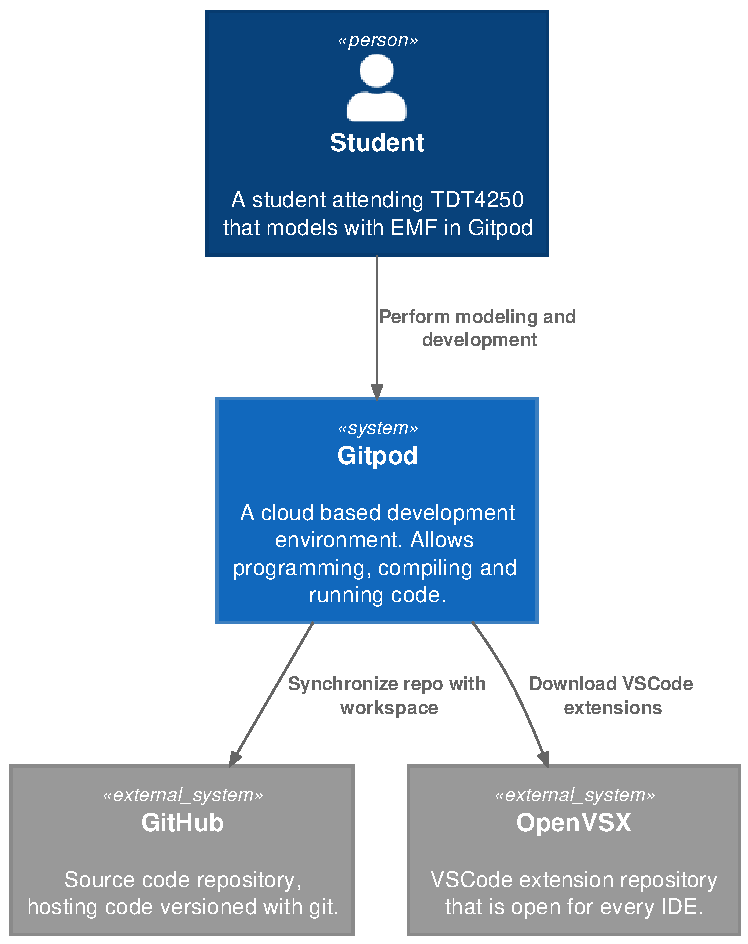
\includegraphics[width=\textwidth]{figures/plantuml/Gitpod_context.pdf}
  \caption[System context diagram for Gitpod]{A system context diagram for Gitpod. The extension will run inside the Gitpod service, used by a student to do modeling and developing. Gitpod uses git to synchronize code with GitHub. The extensions in Gitpod are downloaded from a service called OpenVSX.}\label{fig:gitpod-system-context}
\end{figure}

\begin{figure}[htbp]  % order of priority: h here, t top, b bottom, p page
  \centering
  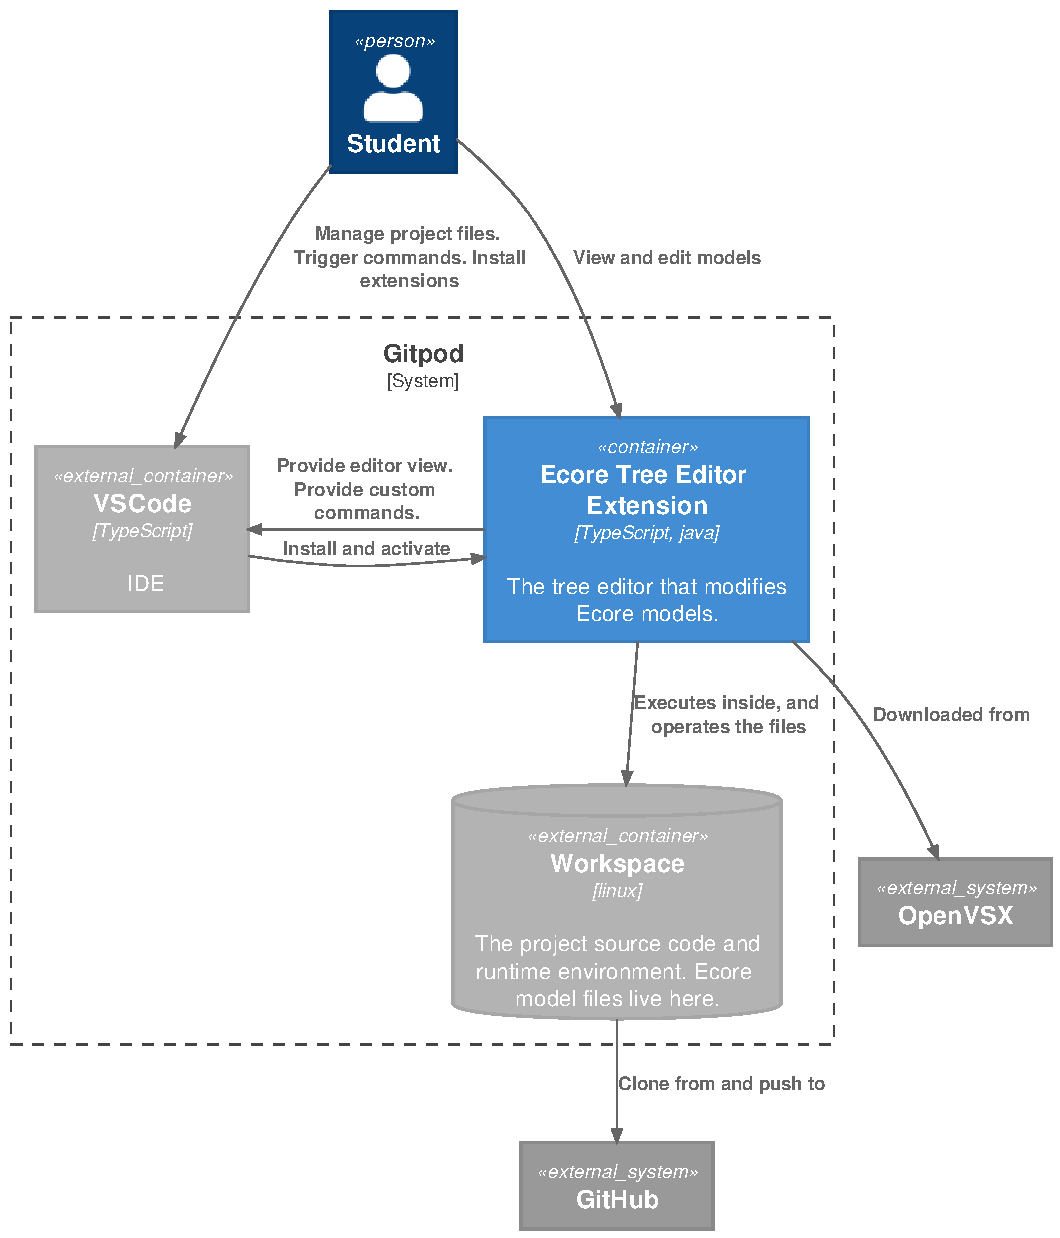
\includegraphics[width=\textwidth,height=\textheight,keepaspectratio]{figures/plantuml/Tree_Editor_Extension_container.pdf}
  \caption[Gitpod container diagram]{Container diagram for gitpod. The Gitpod system from \cref{fig:gitpod-system-context} is expanded to show its internal components. The \acrshort{IDE} used by Gitpod is \gls{Theia}.
  The student will interact with Theia, and install the Ecore Tree Editor Extension created from this thesis.
  This extension will also provide a user interface, which the student uses for modeling.
  This extension reads files from the Gitpod workspace, and uses the runtime provided by the workspace such as a Java Runtime Environment.}\label{fig:gitpod-container-diagram}
\end{figure}

\begin{figure}[htbp]  % order of priority: h here, t top, b bottom, p page
  \centering
  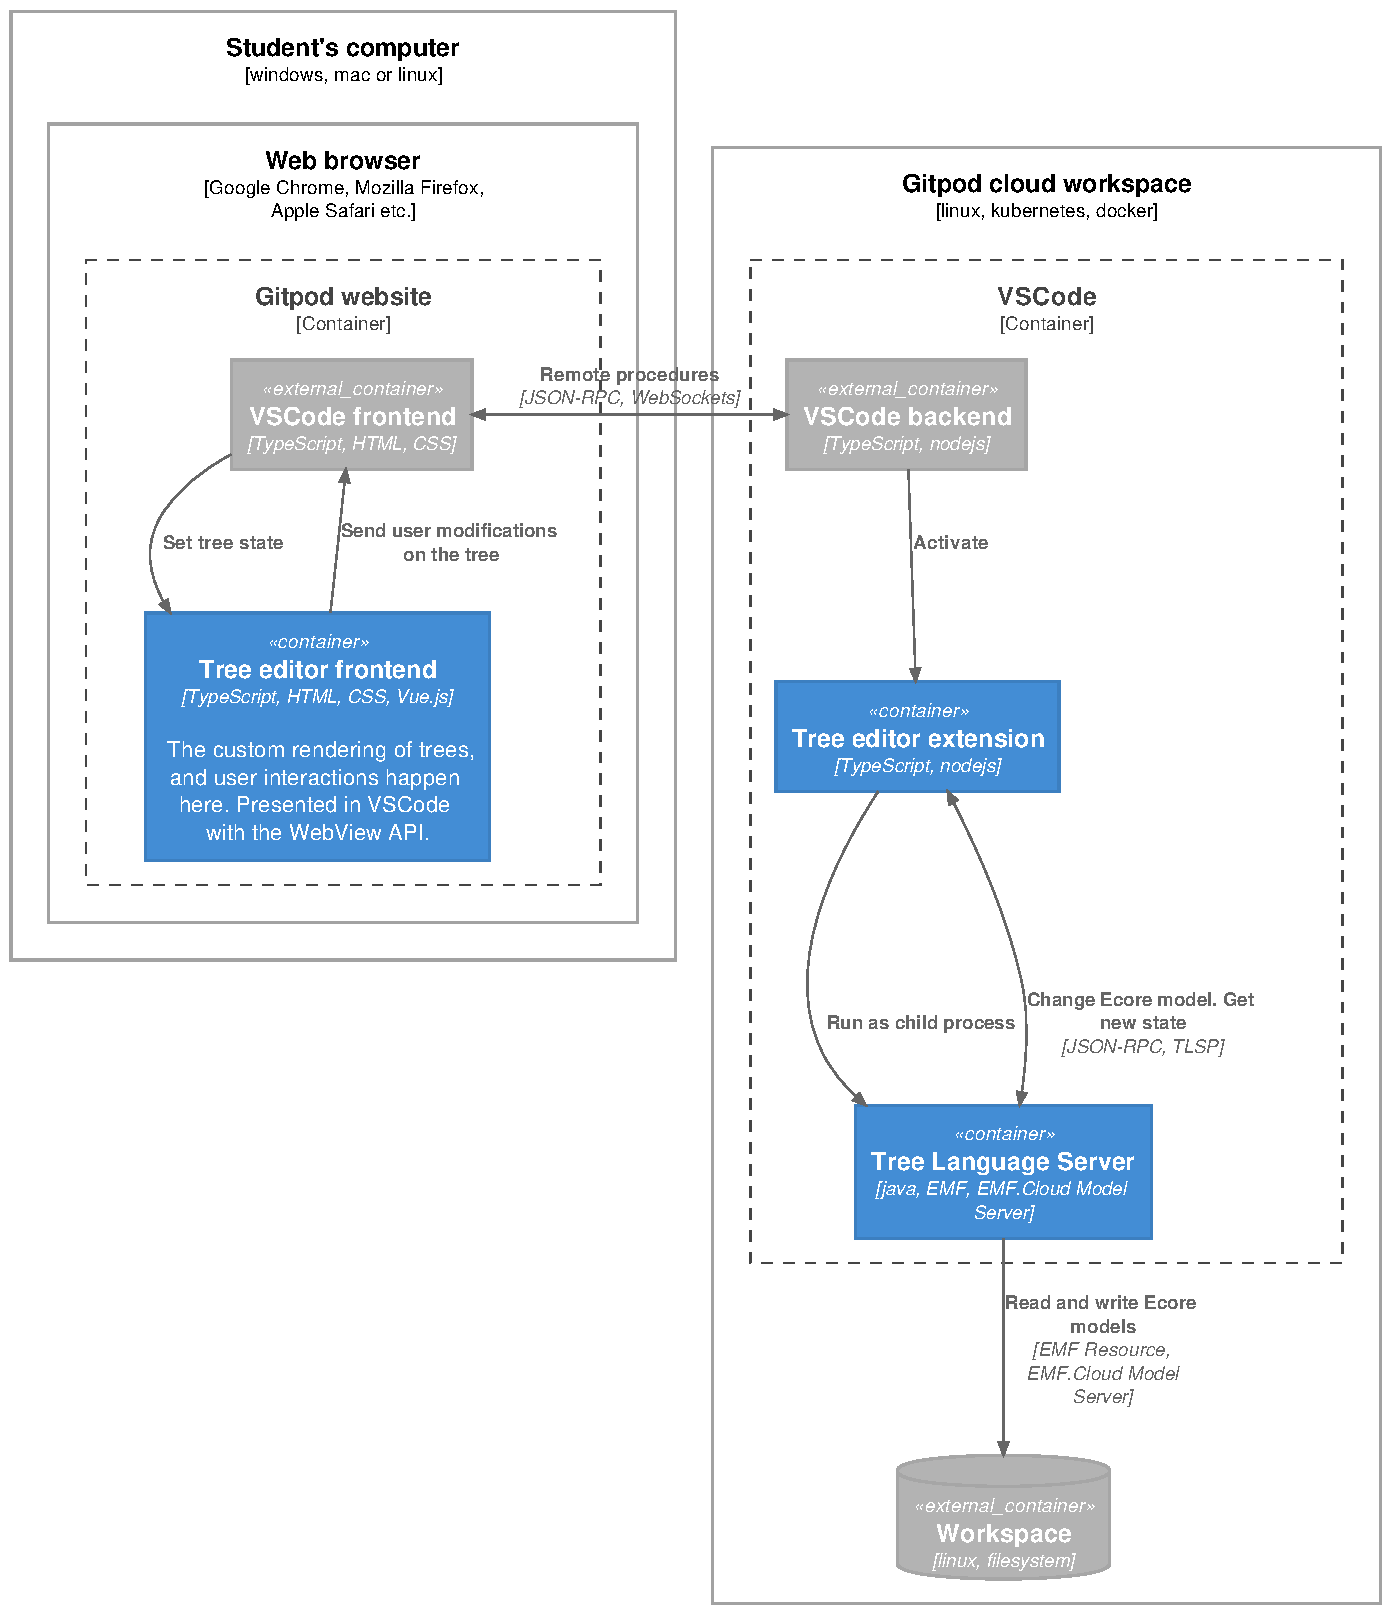
\includegraphics[width=\textwidth,height=\textheight,keepaspectratio]{figures/plantuml/Tree_Editor_Extension_deployment.pdf}
  \caption[Gitpod deployment diagram]{Deployment diagram of Gitpod. The student will use their computer to load the Gitpod website.
  The Gitpod service will start a computer in a cloud provider, to create a cloud workspace.
  The student only loads the Theia frontend and Tree editor frontend into their browser.
  Theia has a backend which runs inside the Workspace, and communicates to the frontend over WebSockets, using JSON-RPC\@.
  The Theia backend will activate the Tree editor extension, which in turn will start a Tree Language Server.
  This Tree Language Server runs java, and reuses the \acrshort{EMF} tooling.
  The Tree editor extension communicates to the Tree Language Server over a well defined protocol, where it asks to read model files, and execute commands to change the models.
  The Tree Language Server uses the Workspace to read and write \texttt{.ecore} files.}\label{fig:gitpod-deployment-diagram}
\end{figure}

\begin{figure}[htbp]  % order of priority: h here, t top, b bottom, p page
  \centering
  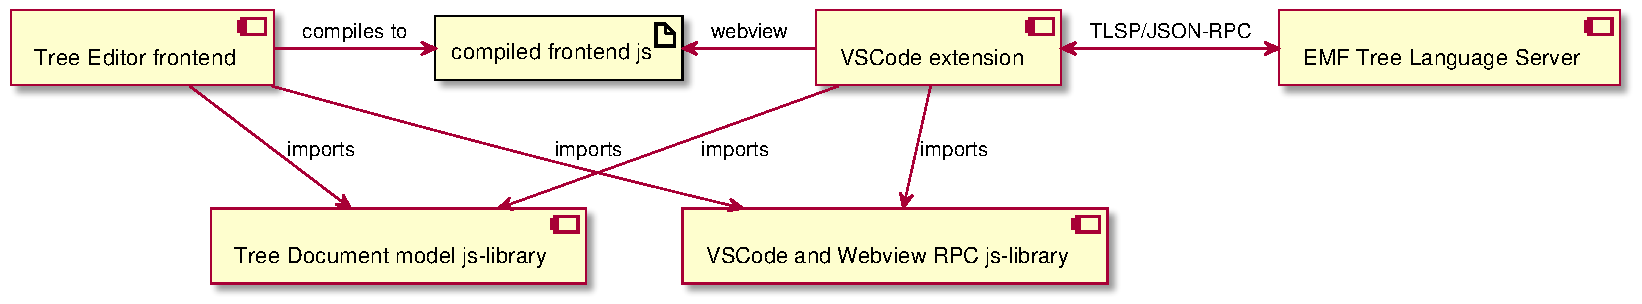
\includegraphics[width=\textwidth]{figures/plantuml/Tree_editor_components.pdf}
  \caption[Ecore Tree Editor component diagram]{Component diagram of the Ecore Tree Editor.
  The for the the extension is organized in 5 separate modules.
  The main module is the VSCode extension.
  This extension bundles the compiled frontend javascript artifact, and the compiled EMF Tree Language Server java jar-file.
  The Tree DOcument model js-library is the layer with the domain model for tree editors.
  It is used in both the frontend and the extension.
  }\label{fig:label4}
\end{figure}

\begin{figure}[htbp]  % order of priority: h here, t top, b bottom, p page
  \centering
  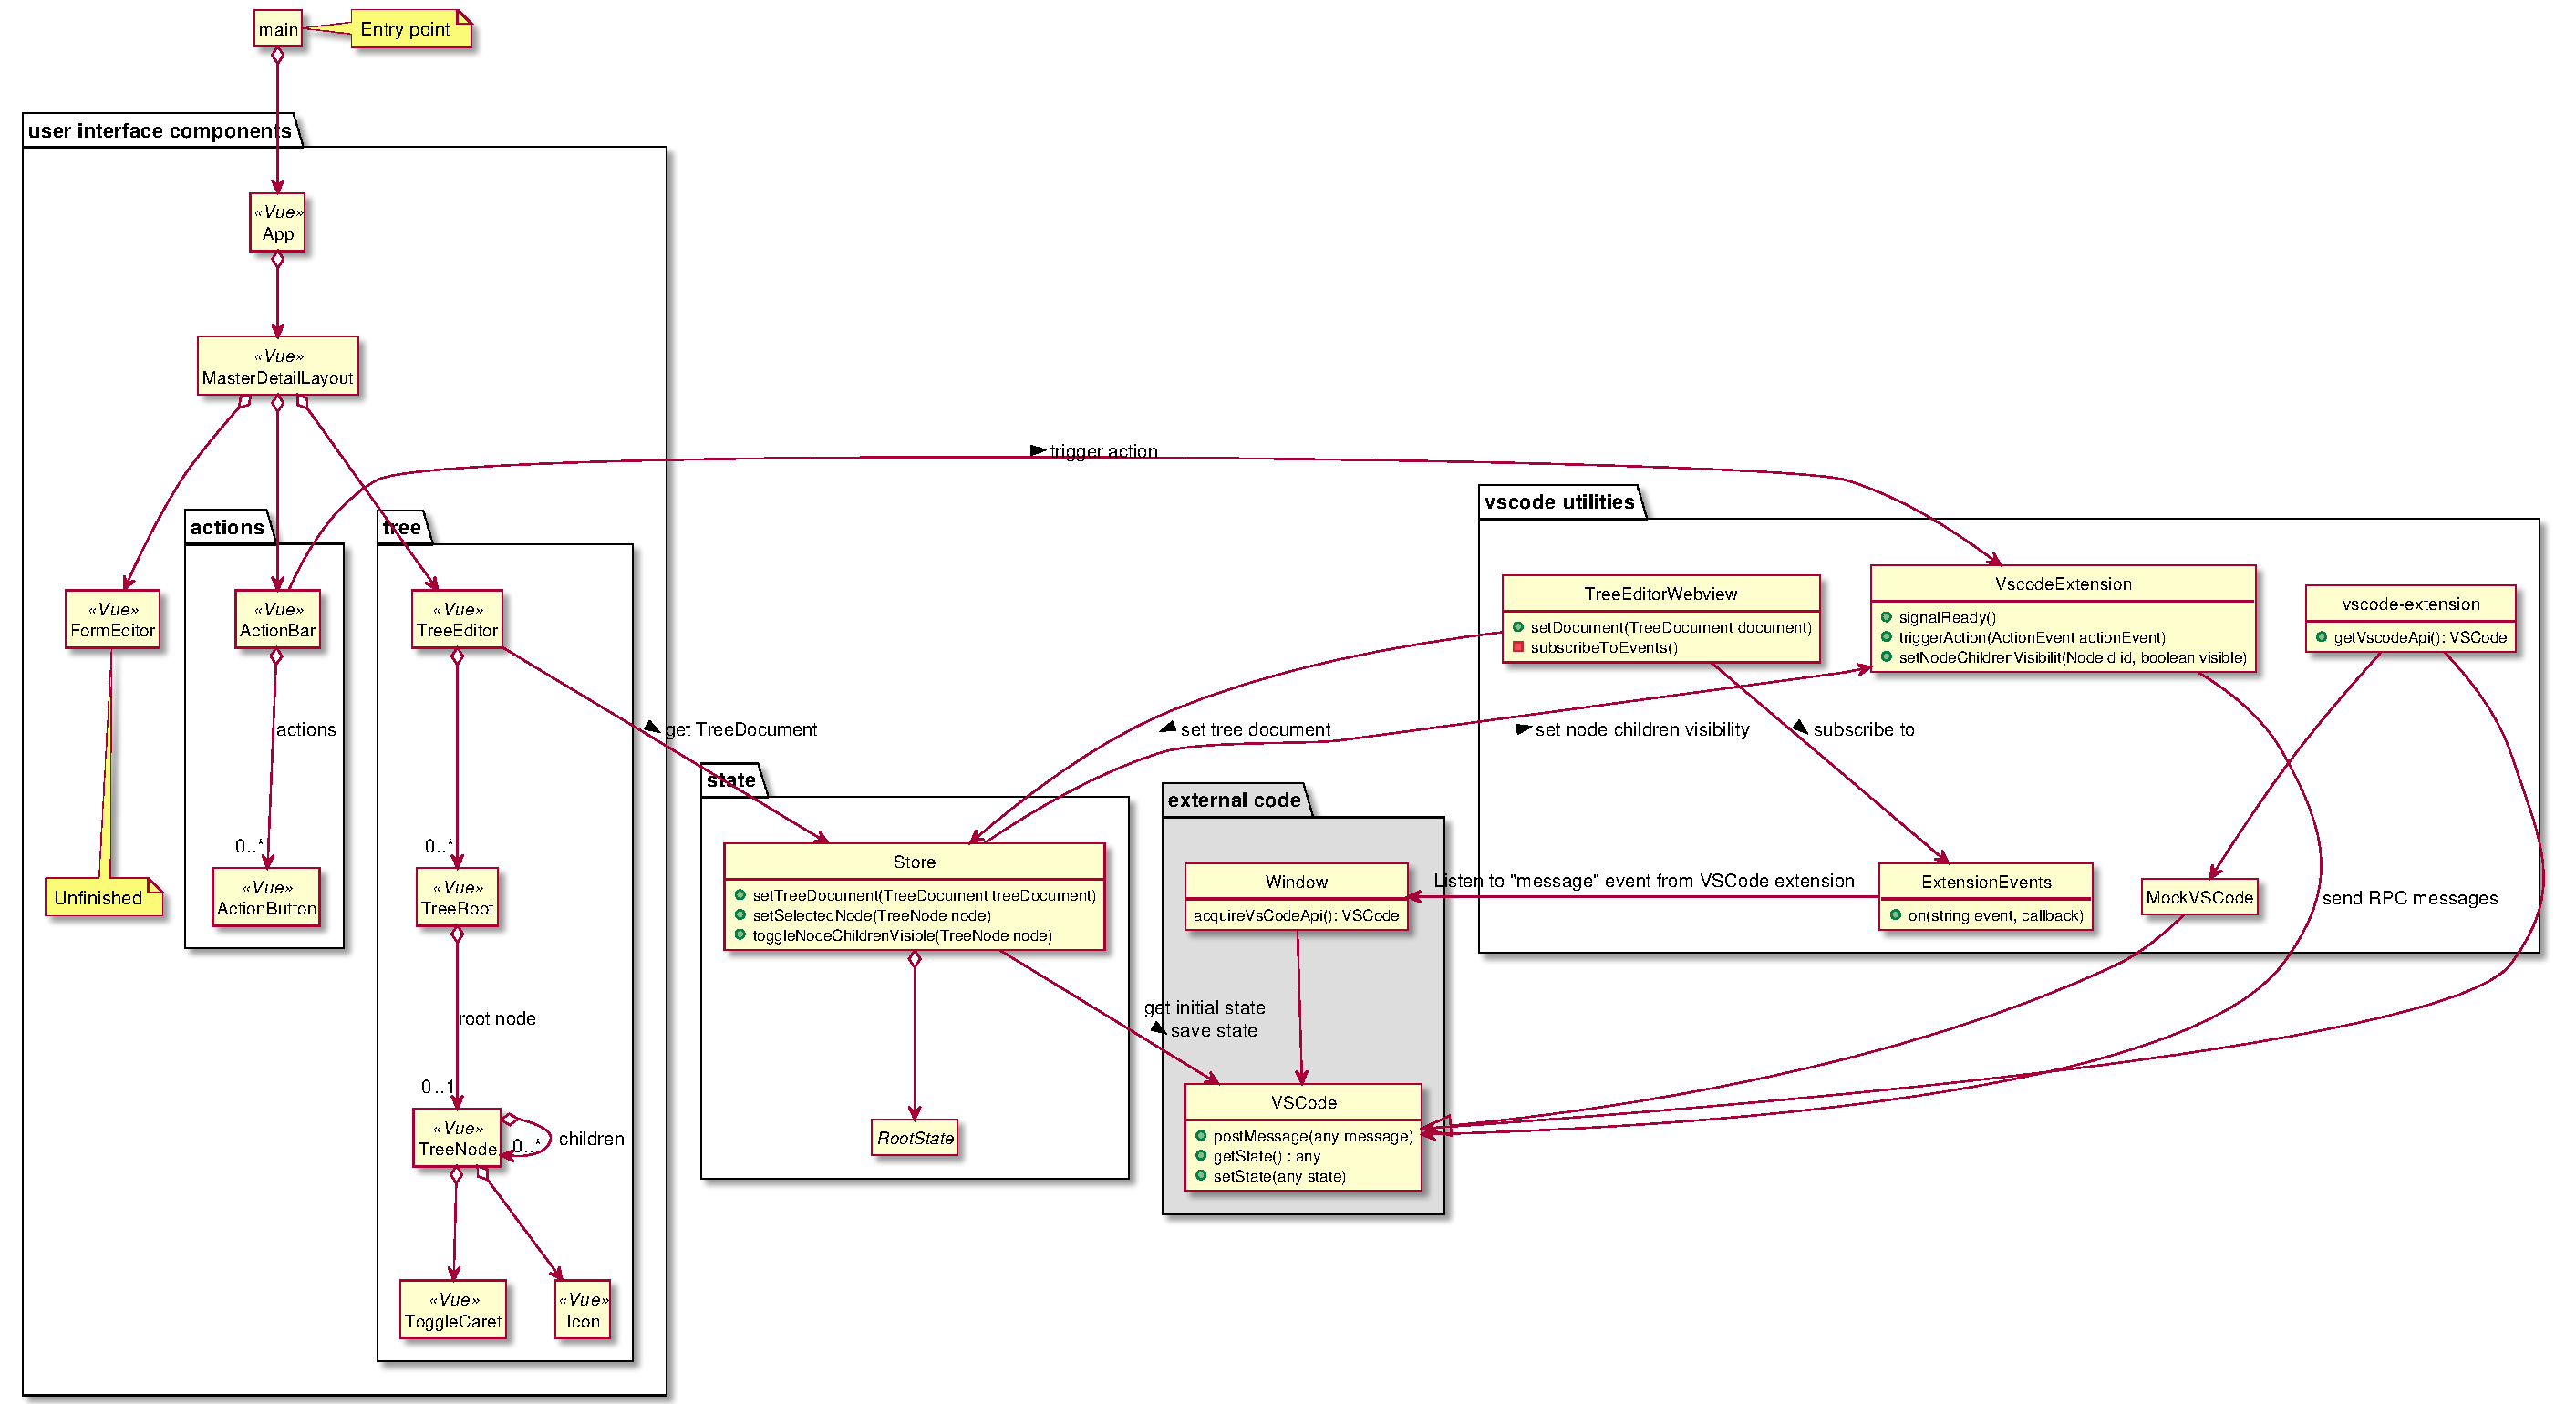
\includegraphics[angle=90,origin=c,width=\textwidth,height=\textheight,keepaspectratio]{figures/plantuml/Tree_Editor_Frontend_code.pdf}
  \caption[Tree Editor Frontend class diagram]{Class diagram of the Tree Editor Frontend component.}\label{fig:tree-editor-frontend-code}
\end{figure}


\begin{figure}[htbp]  % order of priority: h here, t top, b bottom, p page
  \centering
  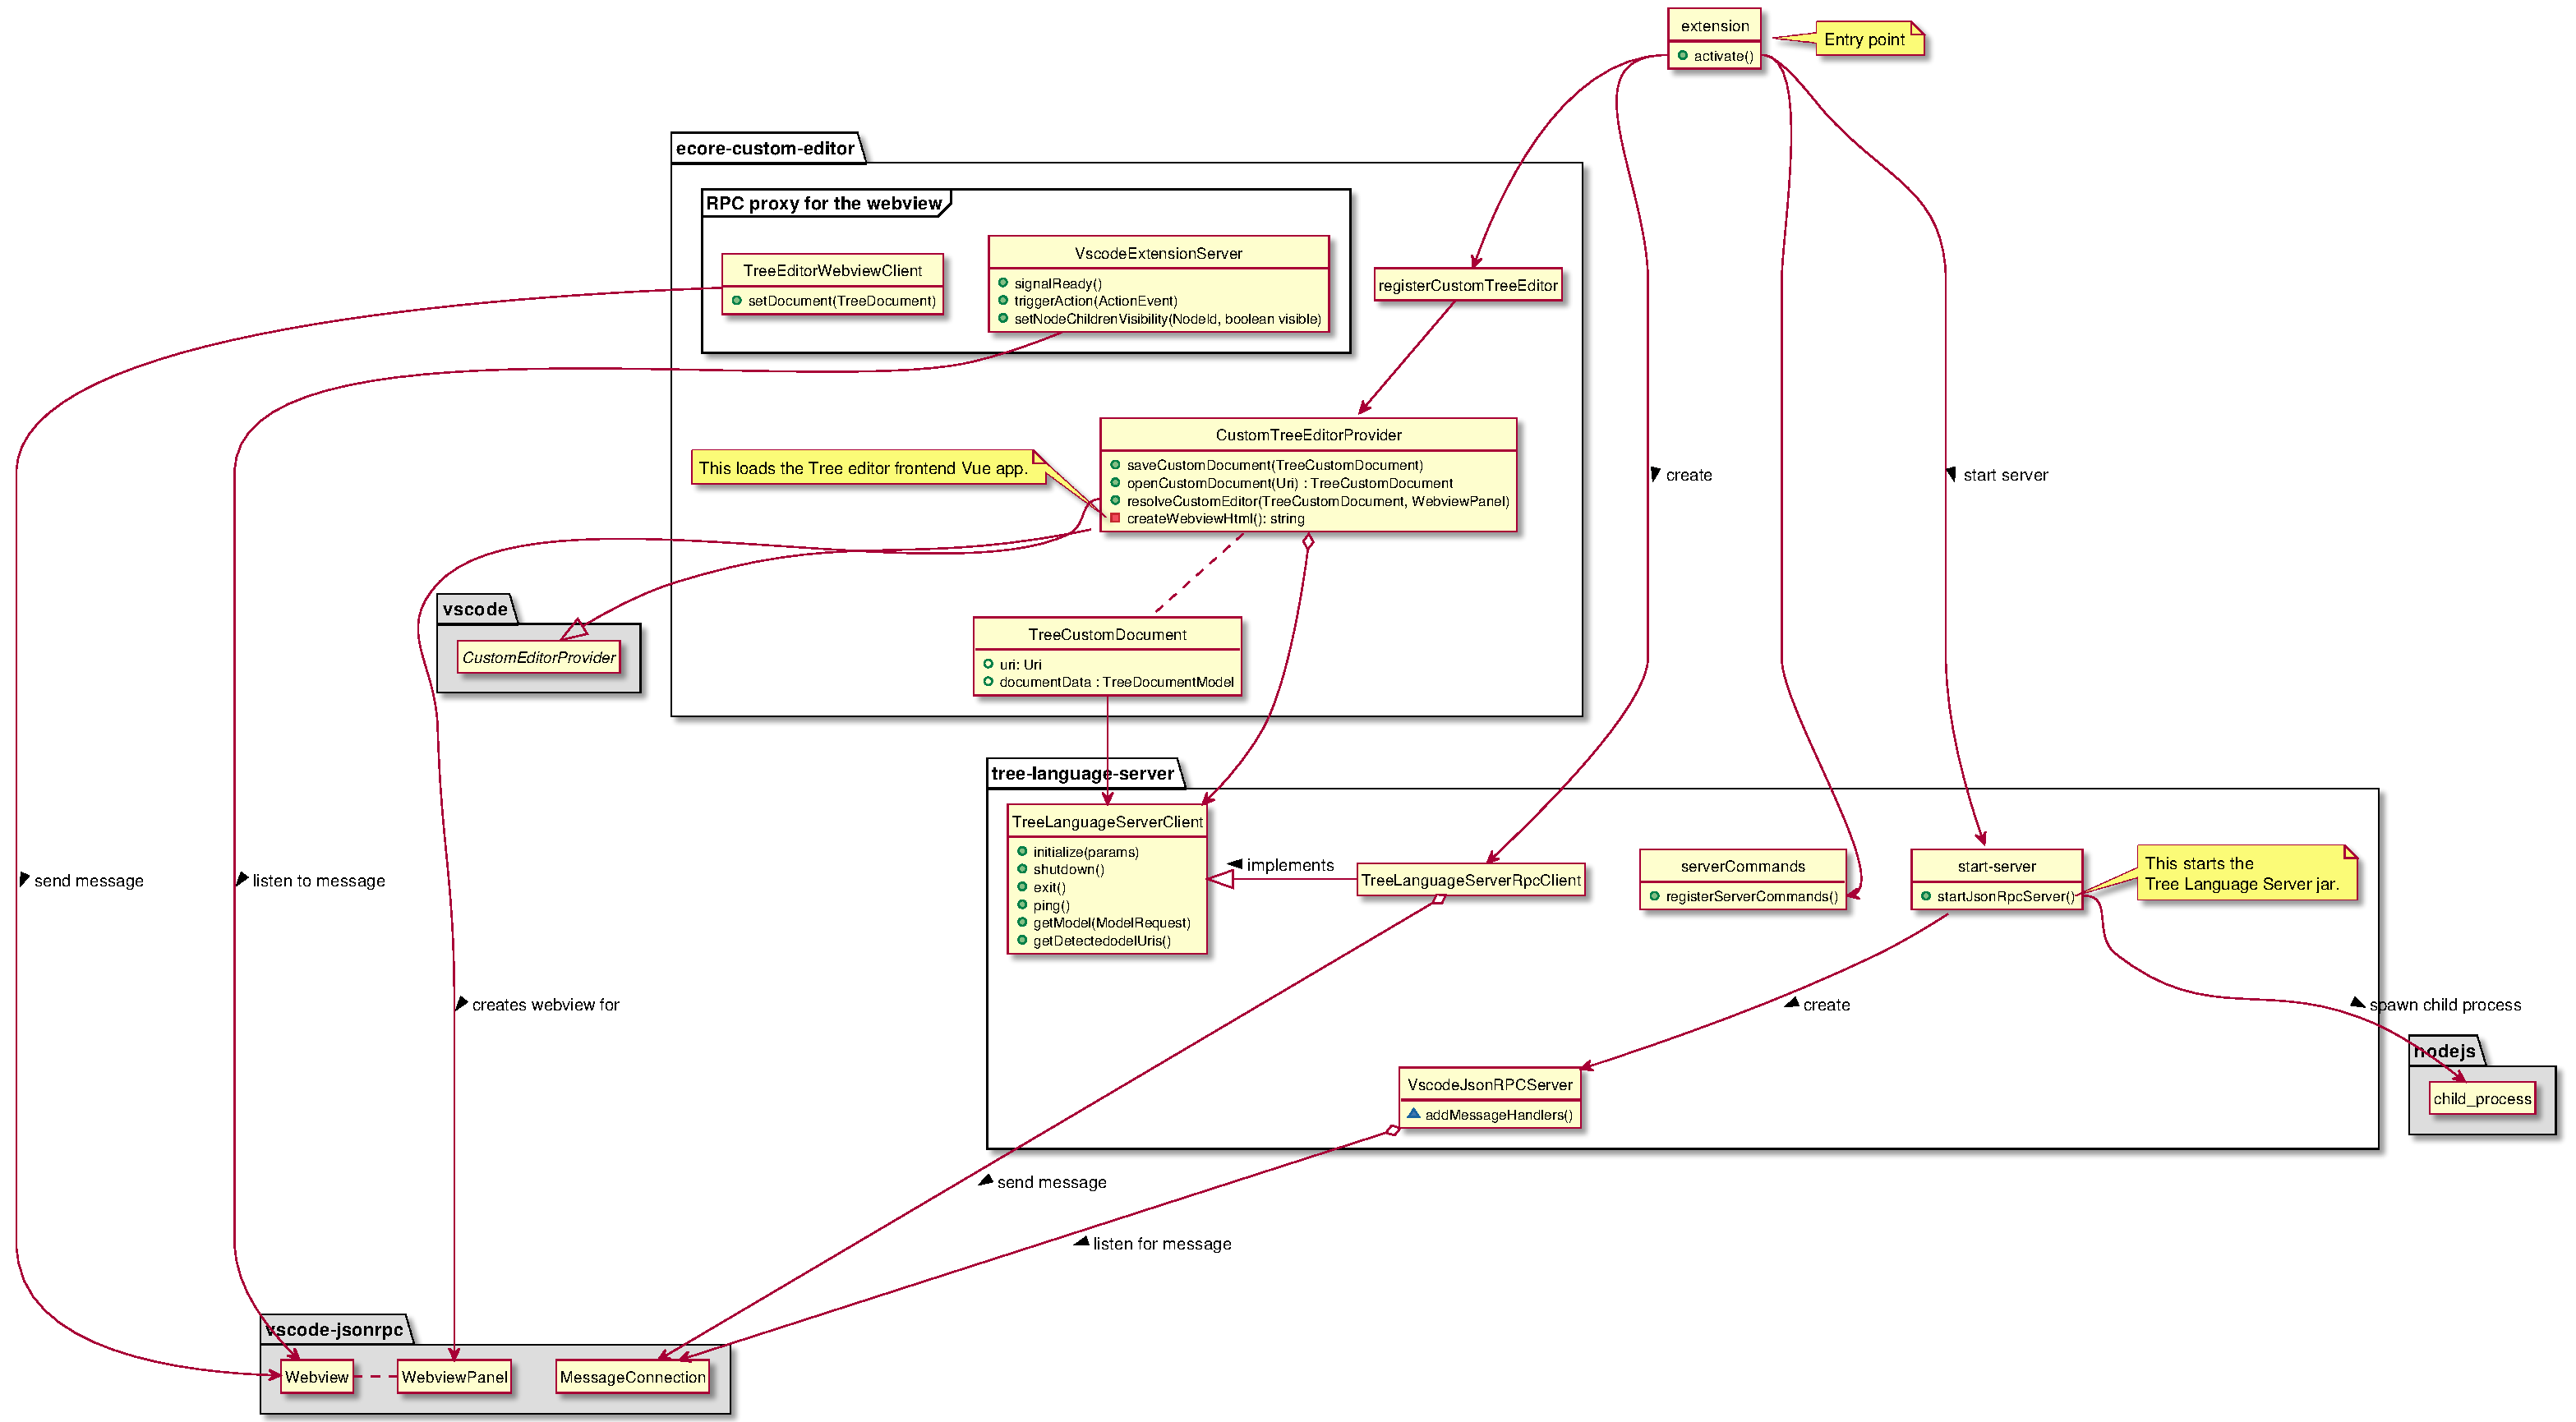
\includegraphics[angle=90,origin=c,width=\textwidth,height=\textheight,keepaspectratio]{figures/plantuml/Tree_Editor_Extension_code.pdf}
  \caption[Tree Editor Extension class diagram]{Class diagram of the Tree Editor Extension component.}\label{fig:label}
\end{figure}


\begin{figure}[htbp]  % order of priority: h here, t top, b bottom, p page
  \centering
  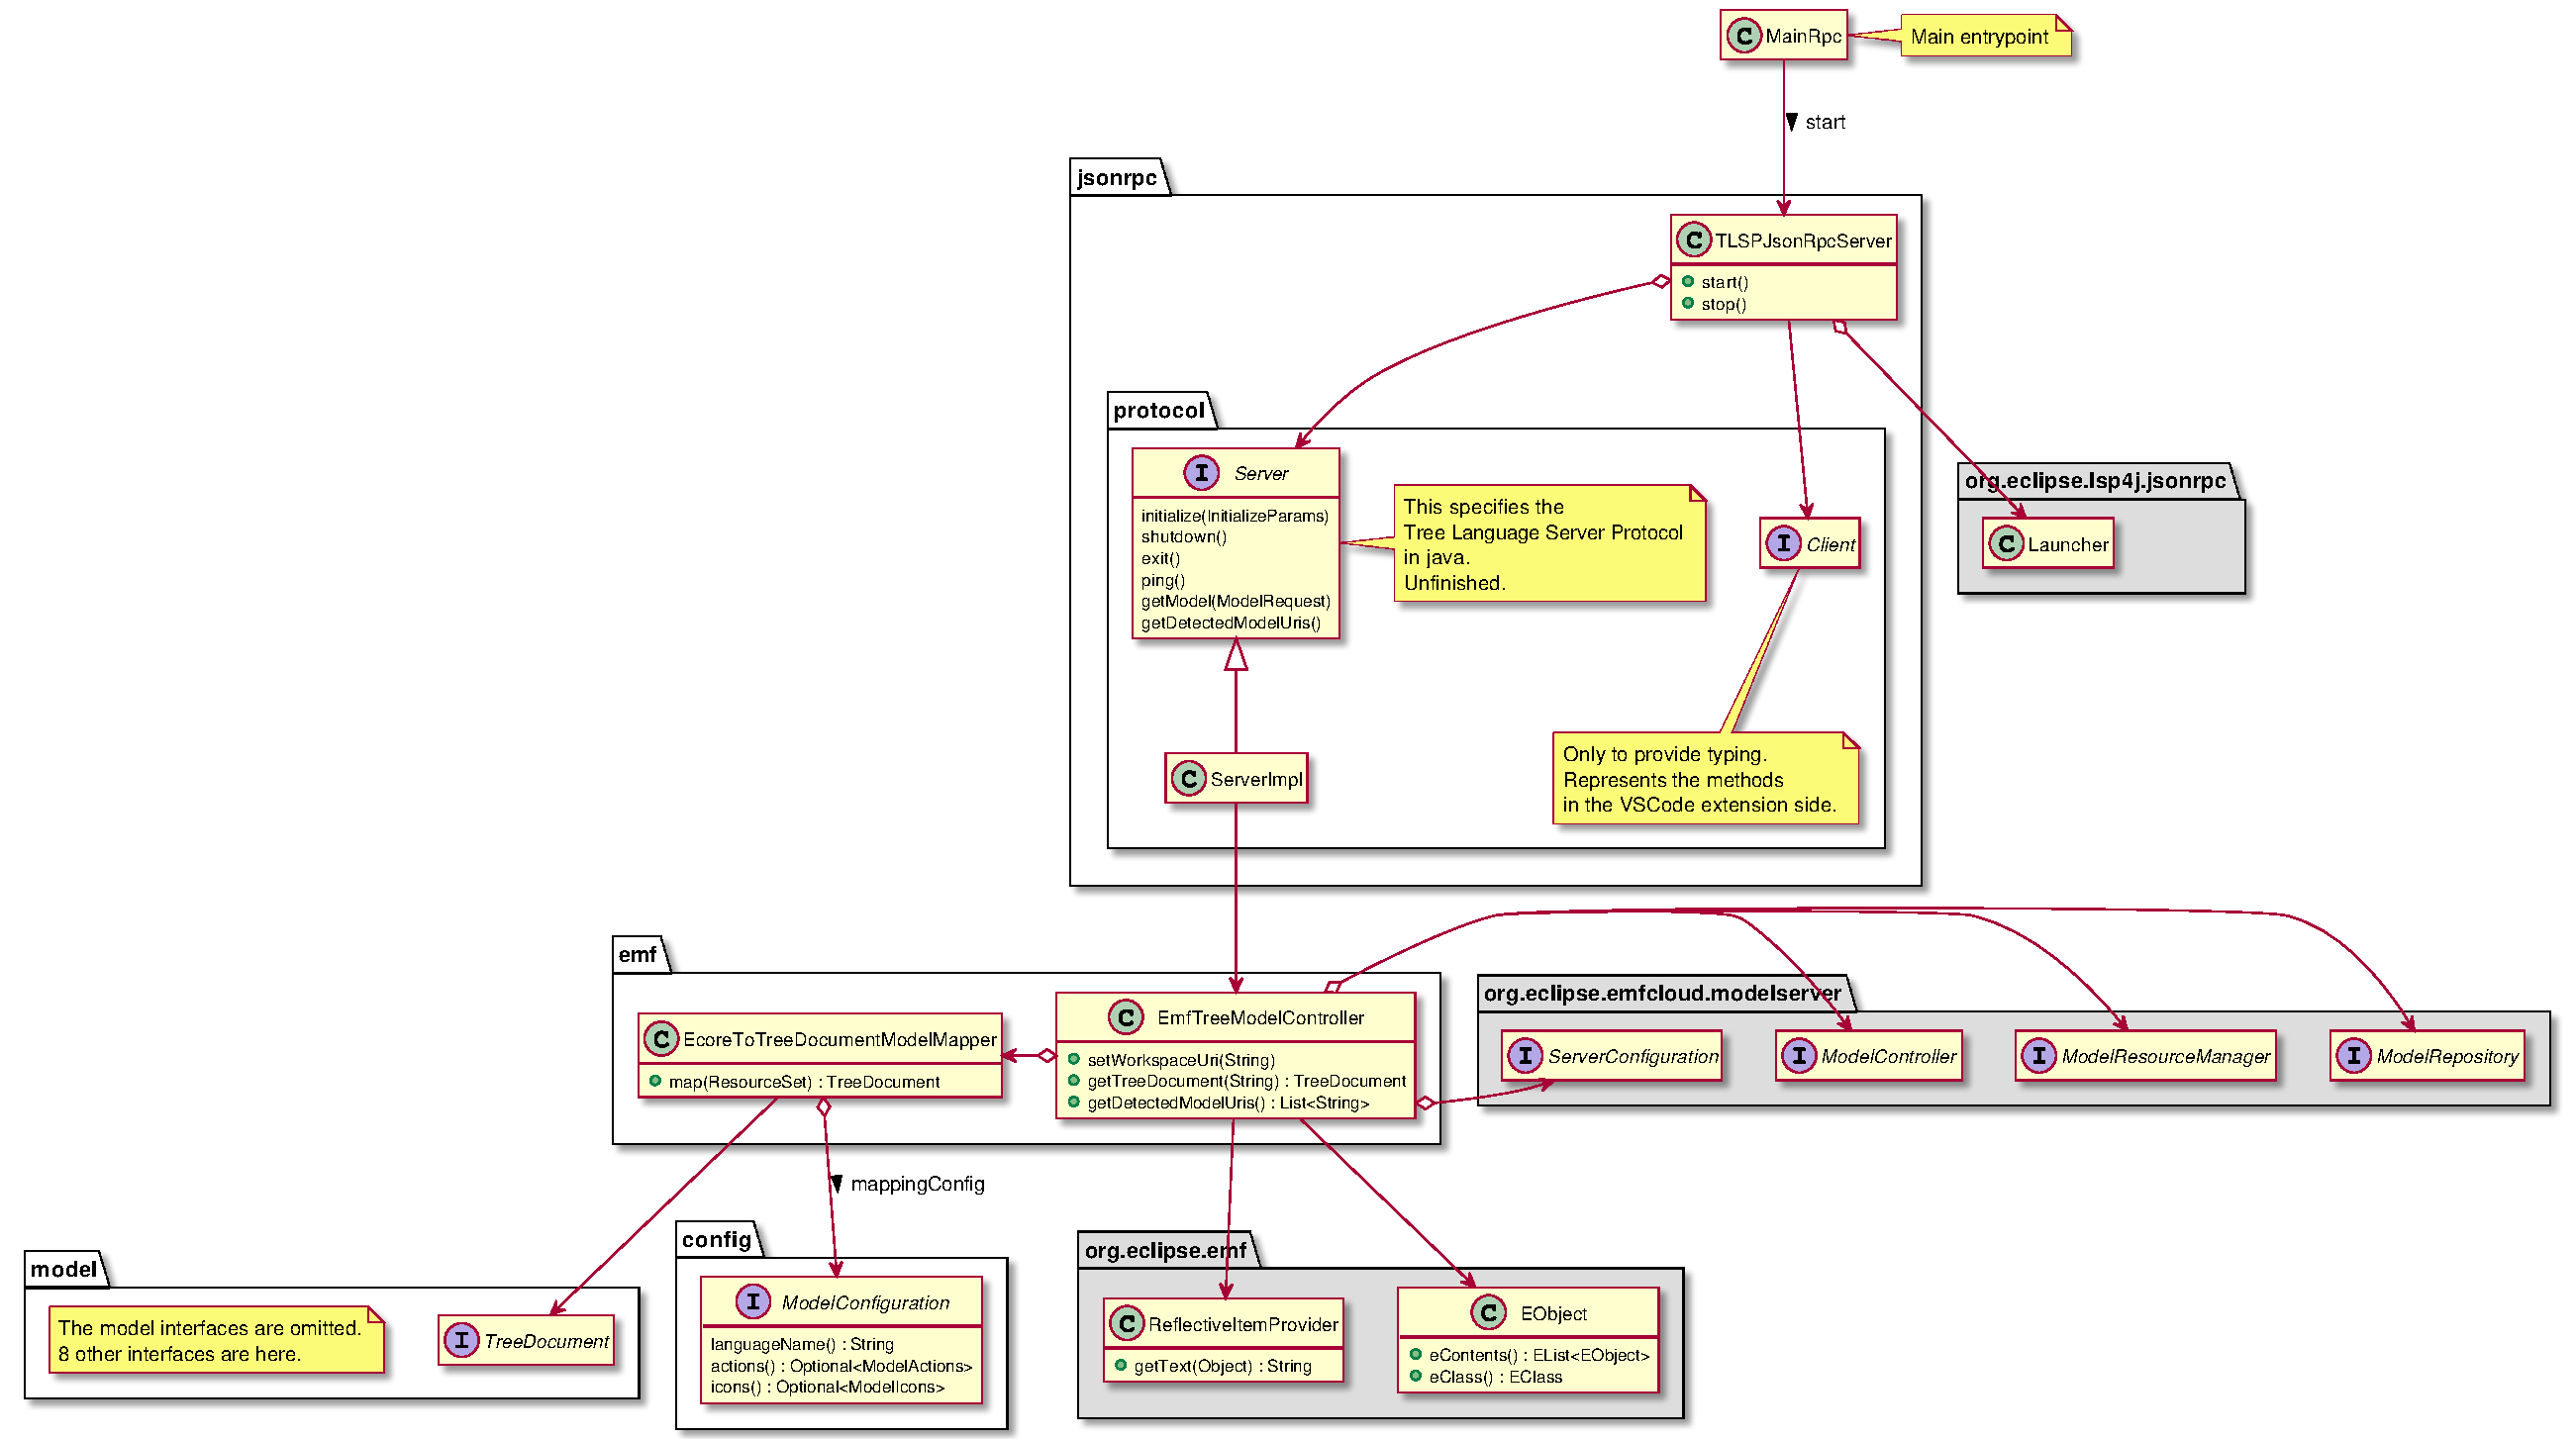
\includegraphics[angle=90,origin=c,width=\textwidth,height=\textheight,keepaspectratio]{figures/plantuml/Tree_Language_Server_code.pdf}
  \caption[Tree Language Server class diagram]{Class diagram of the Tree Language Server component.}\label{fig:label}
\end{figure}